\documentclass[english]{article}
\usepackage[T1]{fontenc}
\usepackage[utf8]{inputenc}
\usepackage{geometry}
\geometry{verbose,tmargin=3.5cm,bmargin=4cm,lmargin=3.8cm,rmargin=3.8cm}

% plots
\usepackage{graphicx}
\graphicspath{ {../plots/} }

% newlines instead of indent for paragraphs
\usepackage[parfill]{parskip}
% tables
\usepackage{multirow}

% import natbib and sets bibliography and citation styles
\usepackage[numbers,sort]{natbib}
\bibliographystyle{apalike}

\makeatletter
\usepackage{hyperref}

\makeatother
\usepackage{babel}

% work in progress packages
\newcommand{\citationneeded}{\textsuperscript{\color{blue} [citation needed]}}
\usepackage{easy-todo}

\begin{document}

\listoftodos

\title{Keep your enemies closer and be loud about it}
\author{Martin Toman}
\date{06 May 2021}
\maketitle

\todo{add supervisor name}
\todo{add contact info and institution}


\begin{abstract}
% The abstract should be short and give the overall idea:
% what is the background, the research questions, what is contribution, and what are the main conclusions.
% It should be readable as a stand-alone text (preferably no references to the paper or outside literature).

\todo{write abstract}
\end{abstract}



\section{Introduction}

% intro - what is prisoner's dilemma
How can we encourage and sustain cooperation? Humans dominate their environments thanks to our ability to cooperate flexibly and at scale, as argued by \citet{harari-sapiens}.
To study the conditions necessary for cooperation to flourish we need a suitable model of an activity with temptations to defect and punishments for doing so.

In 1950, Albert Tucker named a particular two-player exchange game "The Prisoner's Dilemma" \citep{sep-prisoner-dilemma}.
This game elegantly captures the difficulty of the decision between cooperation and defection in a single choice.
Despite being so simple compared to the complexity of the problem it is representing, it was used to model many aspects of behaviour in systems of selfish individuals; and, according to \citet{Axelrod84}, for "discovery of the precise conditions that are necessary and sufficient for cooperation to emerge".

% iterated version + the dilemma
In the case of a one-off exchange, there being no opportunity for a follow-up punishment, the rational behaviour is defection. (This extends to all rounds for a fixed-length game, inductively \citep{Axelrod84}.)
The interesting behaviour arises if there is no end; or, at least, if there is no way for the participants of the game to know when the game ends or even if there is an end.
% reputation importance
An agents has to expect that even a single defection can be infinitely punished by never again being cooperated with \citep{GRIM}.
Such a risk may just not be worth it.

% global reputation system
The defectors can, naturally, only be punished if they can be identified and known to others. This is why services like Ebay or Airbnb have a rating system in place.
Presence of a reputation system has been shown to strongly boost cooperation, as shown by \citet{simple-reputation} and \citet{public-private-monitoring}.
These studies used groups of volunteers as game participants and explored the effects of various information being public - from only the latest move of the current opponent, to full histories of all moves taken by every participant.

% decentralizing reputation: keeping track internally?
These studies were limited by their use of humans as game participants and were thus limited to relatively small groups with few rounds; they also used external infrastructure for information passing: therefore eliminating noise, delays, and deliberately wrong information.
As shown by \citet{noise}, not all strategies that perform well in noise-less environments can do so under the presence of noise.

Using external infrastructure for passing information also meant that the transmission speed was uniform for all participants receiving all necessary information in time for their next round of the game.
These are non-trivial idealizations: relaxing them would yield a model closer to real-world systems and could change the results drastically.

In this paper we look at if and how well a local reputation system sustains cooperation and under what conditions does it yield optimal results.
We evaluate the approach under various gossip range and memory length; and comment on the effectiveness of local reputation in enforcing cooperation in spatial prisoner's dilemma.

\todo{outline the structure of the paper}


\section{Methodology}
We aim to measure the effectiveness of local reputation in enforcing cooperation.
To do this we will build a computer simulation of a spatial multi-agent environment.
We will use a Spatial Iterated Prisoner's Dilemma as the principal exchange game for agent interactions.

In this section we define the goals of this paper explicitly,
explain the design of the model and simulations,
and present the measurable properties and evaluation criteria of the model.
We end the section with explanation of the evaluation criteria and the methods used to draw conclusions from the simulations.

\subsection{Problem Statement}
We will use the prisoner's dilemma game to model the main interaction between the agents.
This is a good choice for observing conditions necessary for cooperation to emerge in a population of rational and selfish agents.
\citationneeded

The agents will live in a spatial environment and act independently;
the only mutual interactions will be playing the game with a neighbor and exchanging gossip with nearby agents.
We will vary the range at which the gossip can be exchanges as well as the amount of information which can be included in as single gossip message.
We want to determine the effectiveness of the gossip mechanism in promoting and sustaining cooperation.

\subsection{Simulation Design}
% Typically in general research articles, the second section contains a description of the research methodology, explaining what you, the researcher, is doing to answer the research question(s), and why you have chosen this method.
% This section includes references to necessary background information.

To explore the effects of local reputation, built up via openly gossiping with local peers, we will use a computer simulation of a multi-agent spatial environment.
We will base the simulation on the design of \citet{smaldino}.

The model consists of a spatial environment:
square grid with torus (wrapping) bounds,
each cell can be occupied by a single agent.
This is a discreet time model;
in each time step, every agent takes a single turn.
The order in which agents take their turn is randomized in each time step.
Agent's turn is defined by a finite state automaton. \todo{add a reference to automaton of agent behaviour}
The agents pay a fixed cost to survive to the next round (agents who deplete their energy die and are removed from the simulation), and try to reproduce once they accumulate enough energy via positive interactions with other agents: game wins.

\todo{add agent behaviour automaton}

Agents reproduce by creating a new agent with the same parameters as themselves in an empty neighborhood cell.
The cost of reproduction is subtracted from the parent and the offspring is birthed with this energy level.
The cost of reproduction is effectively transferred from the parent to the offspring; reproducing does not affect the net amount of energy in the model.

A single round of the game is defined using a payoff matrix as shown in Table \ref{table:payoff}, with $T > R > P > S$ and $2R > T + S$ \citep{chammah1965}.

\begin{table}[h!]
  \centering
  \begin{tabular}{c c||c|c}
    & & \multicolumn{2}{c}{Opponent's move} \\
    & & Cooperate & Defect \\
    \hline\hline

    \multirow{4}{6em}{Player's move}
    & \multirow{2}{5em}{Cooperate}
      & Player:\ \ \ \ \ \ R & Player:\ \ \ \ \ \ S \\
    & & Opponent: R & Opponent: T \\
    \cline{2-4}
    & \multirow{2}{5em}{Defect}
      & Player:\ \ \ \ \ \ T & Player:\ \ \ \ \ \ P \\
    & & Opponent: S & Opponent: P \\
  \end{tabular}

  \caption{Payoff matrix}
  \label{table:payoff}
\end{table}

To better suit our needs we will introduce some changes to the original model.
We will reduce the spatial grid size from 100x100, as in the original design, to a more manageable 20x20.
This will allow us to run more simulations with more complex agent behaviour in a manageable time.
We will also decrease the starting number of agents from 1600 to 64: keeping the same ratio of 16\% of the total grid size as in the original model.

This reduction of the environment size (by a factor of 25!) has the effect of significantly increasing the chance of a total extinction of all agents:
caused by the random behaviour of agents exploiting each other until all cooperators are dead and the population of pure defectors cannot sustain itself.
We disregard runs that end in extinction and increase the number of simulation runs to compensate for this.

We will expand the model by giving the agents a (limited size) memory to keep track of past defectors and later to allow them to actively and freely share this knowledge by gossiping with other agents in a given range.
\todo{add references to related work on memory}

\todo{explain gossip mechanism design}

\subsection{Simulation Evaluation}

To determine the effectives of gossip in enforcing cooperation, we will observe the rate of convergence to a population of cooperators, stopping the simulation once stable equilibrium is achieved. We will also observe the maximal population size of defectors which can sustain itself alongside the cooperators.

\todo{show how we evaluation the effectiveness}

We will also record characteristic patterns formed by the populations as influenced by different parameters. \citationneeded



\section{Results}
% As discussed earlier, in many sciences the methodology is explained in section 2 and this section only discusses the results.
% However, in computer science, most often the details of the evaluation setup are described here first (simulation environment, etc.).
% Very important here is that any skilled reader would be able to reproduce this setup and then obtain the same results.

% Then, results are reported in an accessible manner through figures (preferably with captions that allow them to be understood without going through the whole text), observations are made that clearly follow from the presented results.
% Conclusions are drawn that follow logically from the previous material.
% Sometimes the conclusions are in fact hypotheses, which in turn may give rise to new experiments to be validated.

\begin{figure}[h!]
  \centering
  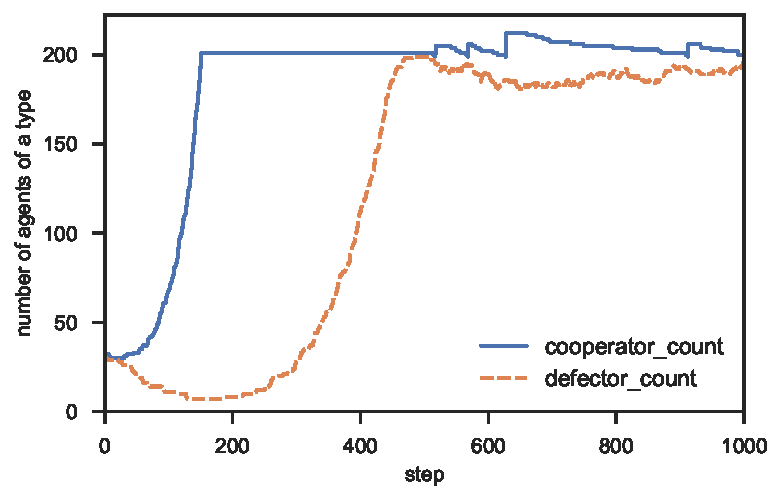
\includegraphics{frequency_time_with_memory.pdf}
  \caption{Evolution of agent population over time (memory size = 1)}
  \label{table:population_evolution}
\end{figure}

\begin{figure}[h!]
  \centering
  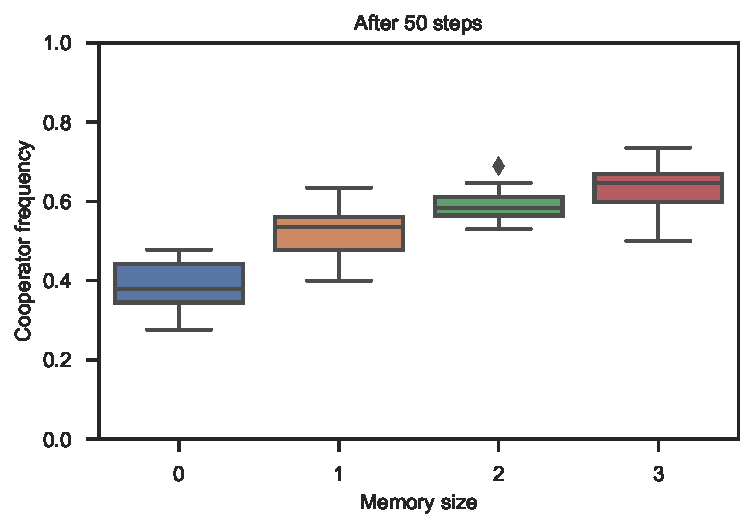
\includegraphics{cooperator_frequency_memory_50steps.pdf}
  \caption{Agent type frequency after $50$ steps}
  \label{table:cooperator_frequency_converged_50}
\end{figure}
\begin{figure}[h!]
  \centering
  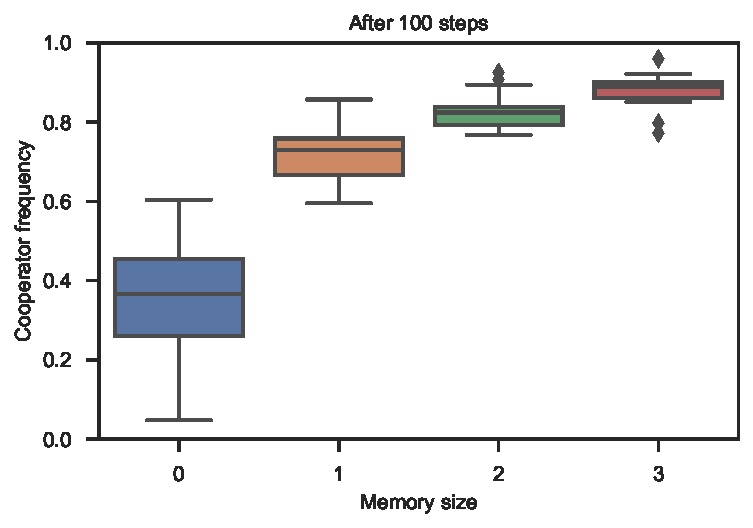
\includegraphics{cooperator_frequency_memory_100steps.pdf}
  \caption{Agent type frequency after $100$ steps}
  \label{table:cooperator_frequency_converged_100}
\end{figure}

% You may want to give this section another name.
\todo{name this section}



\section{Discussion}
% Results can be compared to known results and placed in a broader context.
% Provide a reflection on what has been concluded and how this was done.
% Then give a further possible explanation of results.

% You may give this section another name, or merge it with the one before or the one hereafter.
\todo{write discussion: compare with the human reputation experiment}



\section{Responsible Research}
We recognize the inherent difficulties in conducting ethical and sustainable research.
We take the following actions to ensure this paper is ethically good
and can be reproduced by others, to provide a solid foundation for others to comfortably reproduce, reuse and build upon this paper.

% Reflect on the ethical aspects of your research and discuss the reproducibility of your methods.
\subsection{Ethical aspects}
This paper focused on exploring the effects of reputation on promoting and sustaining cooperation.
We believe this an ethically good research to pursue and our conscience is clean about the methods used and conclusions reach, as well as all other aspects of this paper.

While we cannot ensure the findings of this paper will not be misused by others. We implore all reader's to always strive for the highest ethical goals.
Let's all be excellent.

\subsection{Reproducibility}
We want to make this paper a good foundation for future work and as such we provide all source materials for this paper: including the code files for running the simulations and evaluating results, the \LaTeX\ files for this paper, and anything else used while conducting this research.

Next we use Nix Flake \citationneeded to capture the exact versions of all software, libraries, and packages used for this research. All of this is packaged together and provided as a fully reproducible environment.
We hope that by doing this it becomes easy to reproduce our results and provide a good foundation environment for other researchers to quickly kick-start their research.

Our model itself is implemented in a Jupyter Notebook \citationneeded and care was taken to keep the total amount of dependencies as low as possible and to stick to the most standard dependencies whenever possible.
We hope others will appreciate this by building upon our research and uncovering wonderful conclusions.



\section{Conclusions and Future Work}
% Summarize the research question(s) and the answers to the research question(s).
% Make statements.
% Highlight interesting elements.

% Discuss open issues, possible improvements, and new questions that arise from this work; formulate recommendations for further research.

% ideally, this section can stand on its own: it should be readable without having read the earlier sections.
\subsection{Our conclusions}
\todo{conclude}

\subsection{Future work}
\todo{outline future work: noise, more complex agents, p2p?, make the model public}



\pagebreak
\bibliography{references}

\end{document}
